\chapter{Resultados}

En la siguiente tabla pasamos a mostrar los resultados tanto de la versión anterior de $ISA^{2}$ como de la actual. Como ya dijimos anteriormente, el \ac{MAE} será la métrica que usaremos para esta tarea, pues indica cuánta precisión ha habido en la \ac{SS} realizada por el modelo ``Swiftnet'' \cite{swiftnet} con respecto al modelo ``DeepLab'' \cite{deeplab}.

Recordemos que, a raíz de la \ac{SS} realizada por uno de los modelos, generamos los histogramas que, posteriormente, se usaron en los sistemas de regresión para estimar la velocidad apropiada; de modo que el \ac{MAE} es una métrica muy acertada para saber qué versión del proyecto es mejor.

\begin{table}[H]
\begin{tabular}{|l|l|l|l|l|l|}\hline
& & \multicolumn{2}{|l|}{\textbf{MAE Swiftnet}} & \multicolumn{2}{|l|}{\textbf{MAE DeepLab}} \\ \hline
\textbf{Regresión} & \textbf{Nivel de \ac{SPP}} & \textbf{Highway (\%)} & \textbf{Urban (\%)} & \textbf{Highway (\%)} & \textbf{Urban (\%)}\\ \hline
\multirow{3}{*}{\textbf{\textit{Linear}}} & 1 & 12.22 & 8.95 & 10.32 & 8.38 \\ \cline{2-6}
& 2 & 13.94 & 9.45 & 11.18 & 8.81 \\ \cline{2-6}
& 3 & 13.39 & \textbf{\textit{11.79}} & 15.5 & \textbf{\textit{10.83}}\\ \hline
\multirow{3}{*}{\textbf{\textit{Lasso}}} & 1 & 12.90 & 9.23 & 11.29 & 8.43 \\ \cline{2-6}
 & 2 & 13.80 & 9.40 & 11.7 & 8.62 \\ \cline{2-6}
 & 3 & 13.47 & 10.16 & 10.8 & 9.25\\ \hline
\multirow{3}{*}{\textbf{\textit{Boosting Trees}}} & 1 & 13.43 & \textbf{9.83} & 11.35 & \textbf{10.14} \\ \cline{2-6}
 & 2 & 14.97 & \textbf{10.52} & 12.23 & \textbf{10.72}\\ \cline{2-6}
 & 3 & 14.75 & \textbf{10.08} & 10.37 & \textbf{10.12}\\ \hline
\multirow{3}{*}{\textbf{\textit{SVR}}} & 1 & 11.13 & \textbf{8.74} & 9.69 & \textbf{9.55} \\ \cline{2-6}
 & 2 & 12.24 & \textbf{8.98} & 9.98 & \textbf{9.09}\\ \cline{2-6}
 & 3 & 12.09 & \textbf{9.60} & 9.78 & \textbf{9.62}\\ \hline
\end{tabular}
\caption{Tabla de resultados}
\label{tabla:Resul}
\end{table}

Como se puede apreciar, para cada modelo de \ac{SS} se han segmentado imágenes correspondientes a autovías (o autopistas) y a entornos urbanos.

Los valores de ``Swiftnet'' que aparecen \textbf{resaltados de esta forma} indican que son mejores que los valores de ``DeepLab'' (\textbf{también resaltados}) para esa fila.

Por otro lado, hemos puesto dos valores con \textit{\textbf{este aspecto}} para indicar que, durante la predicción de la velocidad en el sistema de regresión lineal, hemos modificado un parámetro para obtener unos resultados más apropiados; ya que, de otra forma, se obtendrían valores muy lejanos a la realidad.

Como se puede observar, tanto los sistemas \textbf{Boosting Trees} como \ac{SVR} son mejores con la nueva versión para entornos urbanos, mientras que para las autovías es mejor utilizar el modelo ``DeepLab''. Esto quiere decir que ``Swiftnet'' trabaja mejor con entornos en los que se requiere más nivel de detalle y ``DeepLab'', por el contrario, lo realiza mejor en autovías.

Cabe recalcar que ``Swiftnet'' \cite{swiftnet} es un modelo ``Real-Time'', de modo que su implementación es menos que costosa que ``DeepLab, el cual, por el contrario, necesita de un tiempo de procesamiento para realizar su función.

A continuación mostramos algunas figuras con las que podemos ver, de forma gráfica, los resultados de los sistemas de regresión con la \ac{SS} realizada por ``Swiftnet'':

\begin{figure}[H]
  \centering
  \begin{subfigure}[b]{0.45\linewidth}
    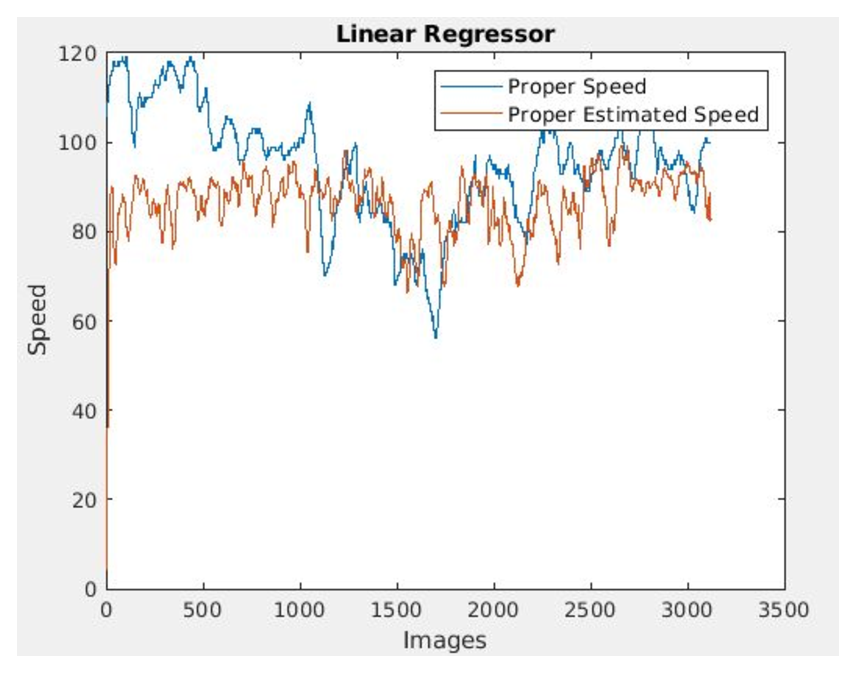
\includegraphics[width=\linewidth]{Figuras/Lineal_Highway(Nivel_1).eps}
    \caption{Highway con Lineal en nivel 1 de \ac{SPP}}
  \end{subfigure}
    \begin{subfigure}[b]{0.425\linewidth}
    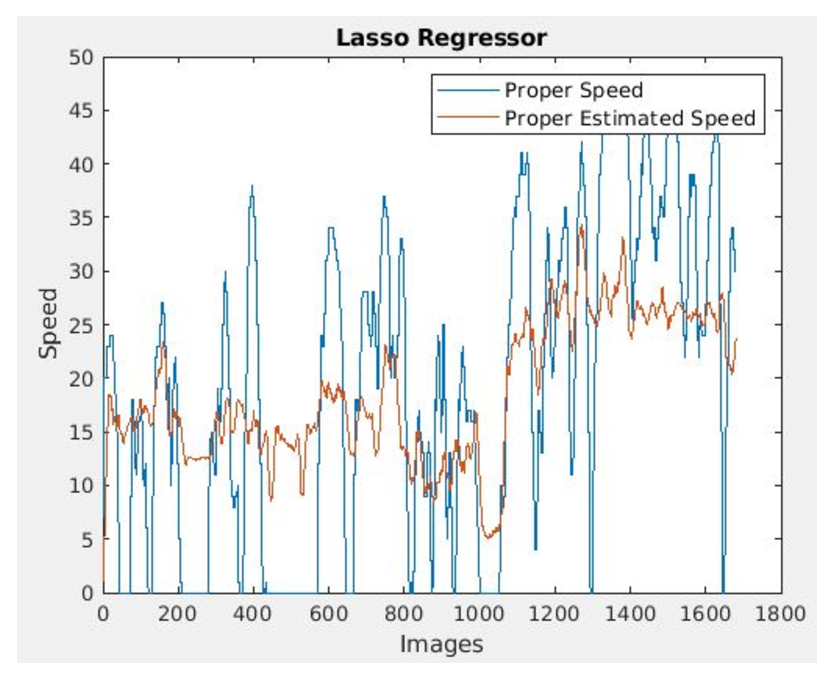
\includegraphics[width=\linewidth]{Figuras/Lasso_Urban(Nivel_1).eps}
    \caption{Urban con Lasso en nivel 1 de \ac{SPP}}
  \end{subfigure}
    \begin{subfigure}[b]{0.45\linewidth}
    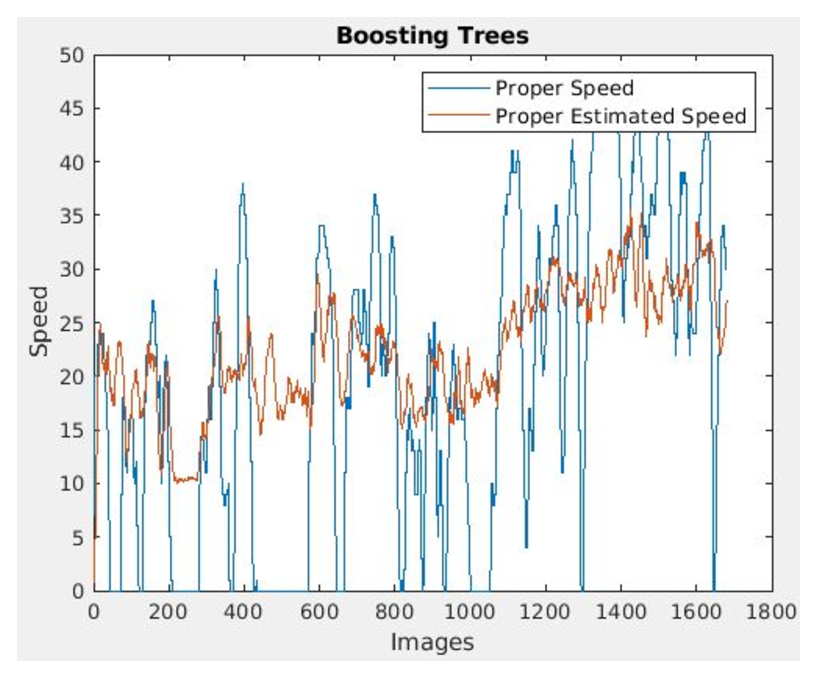
\includegraphics[width=\linewidth]{Figuras/Boosting_Urban(Nivel_1).eps}
    \caption{Urban con Boosting en nivel 1 de \ac{SPP}}
  \end{subfigure}
      \begin{subfigure}[b]{0.45\linewidth}
    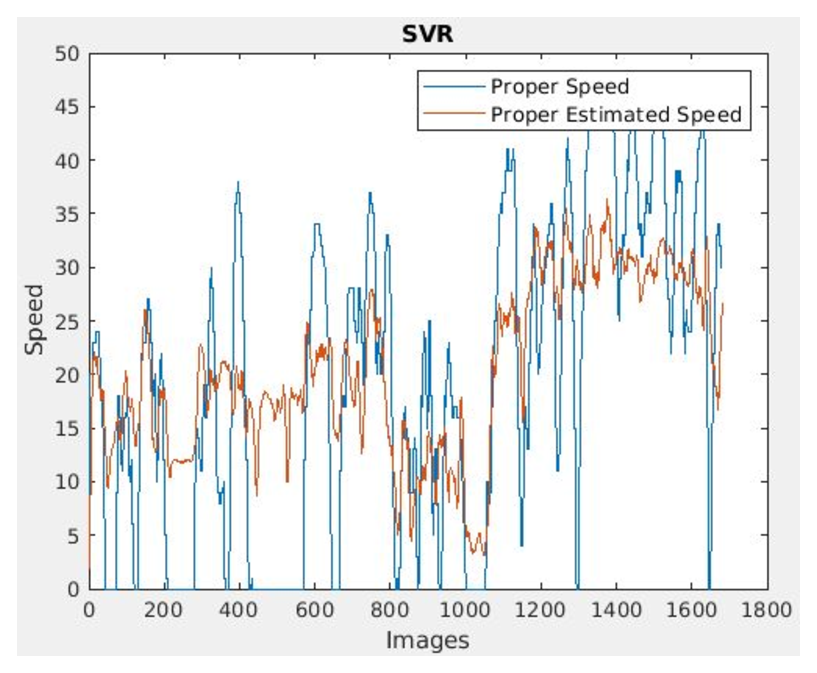
\includegraphics[width=\linewidth]{Figuras/SVR_Urban(Nivel_1).eps}
    \caption{Urban con SVR en nivel 1 de \ac{SPP}}
  \end{subfigure}
  \caption{Resultados gráficos}
\end{figure}

Hemos visto cómo se realiza todo el proceso de este trabajo y hemos comparado los resultados actuales con los anteriores. A continuación, finalizaremos con las conclusiones de éste.